\def\year{2022}\relax
\documentclass[letterpaper]{article} % DO NOT CHANGE THIS
\usepackage{aaai22}  % DO NOT CHANGE THIS
\usepackage{times}  % DO NOT CHANGE THIS
\usepackage{helvet}  % DO NOT CHANGE THIS
\usepackage{courier}  % DO NOT CHANGE THIS
\usepackage[hyphens]{url}  % DO NOT CHANGE THIS
\usepackage{graphicx} % DO NOT CHANGE THIS
\urlstyle{rm} % DO NOT CHANGE THIS
\def\UrlFont{\rm}  % DO NOT CHANGE THIS
\usepackage{natbib}  % DO NOT CHANGE THIS AND DO NOT ADD ANY OPTIONS TO IT
\usepackage{caption} % DO NOT CHANGE THIS AND DO NOT ADD ANY OPTIONS TO IT
\DeclareCaptionStyle{ruled}{labelfont=normalfont,labelsep=colon,strut=off} % DO NOT CHANGE THIS
\frenchspacing  % DO NOT CHANGE THIS
\setlength{\pdfpagewidth}{8.5in}  % DO NOT CHANGE THIS
\setlength{\pdfpageheight}{11in}  % DO NOT CHANGE THIS
\usepackage{algorithm}
\usepackage{algpseudocode}
\usepackage{amssymb}
\usepackage{amsmath}
\usepackage{xcolor}
\usepackage{amsthm}
\usepackage{adjustbox}
\usepackage{multirow}

\usepackage{enumitem}
\newlist{myitemize}{itemize}{1}
\setlist[myitemize,1]{label=\textbullet,leftmargin=0pt}

\newtheorem{definition}{Definition}
\newtheorem{theorem}{Theorem}[section]
\newtheorem{lemma}[theorem]{Lemma}
\usepackage{newfloat}
\usepackage{listings}
\lstset{%
	basicstyle={\footnotesize\ttfamily},% footnotesize acceptable for monospace
	numbers=left,numberstyle=\footnotesize,xleftmargin=2em,% show line numbers, remove this entire line if you don't want the numbers.
	aboveskip=0pt,belowskip=0pt,%
	showstringspaces=false,tabsize=2,breaklines=true}
\floatstyle{ruled}
\newfloat{listing}{tb}{lst}{}
\floatname{listing}{Listing} 

\pdfinfo{
/Title (Considering Theory of Mind in  Human-Aware Task Planning for a Collaborative Robot)
/Author Paper #8284)
/TemplateVersion (2022.1)
}

\setcounter{secnumdepth}{0} %May be changed to 1 or 2 if section numbers are desired.

\title
{
Will They Know? Integrating Theory of Mind \\ in Human Aware Task Planning for Collaborative Robots
}
\author{
    %Authors
    % All authors must be in the same font size and format.
    % Anthony Favier\textsuperscript{\rm 1,2},
    % Shashank Shekhar\textsuperscript{\rm 1},
    % Rachid Alami\textsuperscript{\rm 1,2}
    Authors
}
\affiliations{
    % Afiliations
    % \textsuperscript{\rm 1}LAAS-CNRS, Universite de Toulouse, Toulouse, France\\
    % \textsuperscript{\rm 2}{Artificial and Natural Intelligence Toulouse Institute (ANITI)}

    % % email address must be in roman text type, not monospace or sans serif
    % \{anthony.favier, sshekhar, rachid.alami\}@laas.fr
    % Affiliations
}

\begin{document}

%%%%% SYMBOLS DEFINITION %%%%%
\newcommand{\worldstates}{\mathcal{S}}
\newcommand{\worldstate}{s}
\newcommand{\fluent}[3]{\mathcal{F}^{#1#2}_{#3}}
\newcommand{\prop}{\varphi}
\newcommand{\allprops}{\Phi}
\newcommand{\predicate}{\mathcal{P}}
\newcommand{\predval}{v}
\newcommand{\agent}{\lambda}
\newcommand{\beliefs}{\mathcal{B}}
\newcommand{\human}{H}
\newcommand{\robot}{R}
\newcommand{\places}{\mathcal{P}}
\newcommand{\place}{p}
\newcommand{\unknown}{UnKw}
\newcommand{\known}{Kw}
\newcommand{\missedactions}{\mathcal{M}}
\newcommand{\loc}[1]{loc(#1)}
\newcommand{\obs}[1]{obs(#1)}
\newcommand{\dom}[1]{dom(#1)}
\newcommand{\observable}{\texttt{OBS}}
\newcommand{\inferable}{\texttt{INF}}
%%%%%%%%%%%%%%%%%%%%%%%%%%%%%%

\maketitle

\begin{abstract}

It is essential for a collaborative robot to consider Theory of Mind (ToM) when interacting with humans. Several works integrate ToM when executing joint plans to adapt online the robot's behavior to unplanned human initiatives. 
However, having such considerations while planning offline for the robot by taking humans' behaviors into account; can offer it smarter and more proactive alternatives.
Recent offline planning schemes like HATP/EHDA explicitly model humans as \textit{uncontrollable} agents and aim to plan for robot's actions while coordinating them \textit{implicitly} with the estimated human's behaviors. These schemes are suitable for and would benefit from integrating ToM concepts in a principled way to anticipate human behavior better.
In this paper, based on an existing scheme, we propose a new contribution --- an offline planning approach allowing for better estimation and exploitation of the human's mental state. 
More precisely, our approach formalizes for each agent simple yet elegant situation assessment models, which are managed at the symbolic level and inserted in the planning process. They are based on the notion of {\em co-presence}
and two types of action effects: (1) facts that are inferred while performing an action or observing an action being executed, and (2) facts that can be observed by an agent at any time. Thanks to this addition, we show how ambiguous situations due to estimated false human beliefs are detected and can be avoided by different means (communication or delayed robot actions).
We implemented our new conceptual approach, prove its soundness and completeness, discuss its effectiveness qualitatively, and show experimental results on three novel domains.

\end{abstract}

\section{Introduction}
Human-Robot Collaboration (HRC) is a current research focus due to the growing number of robot-assisted applications~\cite{kragic2021effective,selvaggio2021autonomy}. Collaborative robots add clear value to manufacturing by promising to boost productivity and improve working conditions~\cite{johannsmeier2016hierarchical}. In assembly lines, there is a strong economic advantage to allowing robots and humans to collaborate~\cite{nikolaidis2012human,coupete2015gesture}. Therefore, a certain amount of autonomy from the robot's side is quite beneficial with respect to the collaboration's efficiency and efficacy.  
However, integrating collaborative robots in human workplaces is non-trivial and primarily raises two types of research challenges: (1) perceiving human behavior and predicting their intended goals/tasks \cite{cheng2020towards,cheng2019human}, and (2) planning for the robot's behavior while also considering humans' behavior, which is also broadly known as human-aware decision making and planning~\cite{CirilloKS09a,alami2006toward,CirilloKS09,de2015hatp,CramerKD21,unhelkar2020decision}, and negotiating for role allocation~\cite{roncone2017transparent}. 
In this paper we focus on the latter challenge, and in particular, human aware interaction planning for a subclass of human-robot collaborative tasks, namely sequential tasks with known joint task objectives~\cite{cheng2021human,UnhelkarLS19,buisan:hal-03684211}, which can be applied in various domains like assembly line~\cite{unhelkar2018human}, in supporting human surgeons~\cite{jacob2013collaboration}, and astronauts~\cite{diftler2011robonaut}. 

For a seamless human-robot collaboration, it is essential to integrate a task planning framework~\cite{lallement2018hatp} and/or a behavior scheduling framework~\cite{ferreira2021scheduling} and an online joint behavior execution scheme. In~\cite{PupaS21}, updated planning information is dynamically integrated into the scheduling framework, while Devin and Alami~(\citeyear{devin2016implemented}) (henceforth, DA) propose to consider ToM when interacting with humans to react to their \textit{unplanned} run-time initiatives,
e.g., their temporary absence or inattention, which prohibit humans from entailing the exact execution status. 
However, replanning frameworks generally come with a supervisor as in~\cite{johannsmeier2016hierarchical} or DA's, which
reduces flexibility and makes humans more
stressed as, roughly speaking, the robot routinely communicates by asking or requesting new information like new ground truths, refined plans, etc.

Recently proposed planning frameworks as in~\cite{buisan:hal-03684211,UnhelkarLS19} provide more flexibility to the human. These offline approaches accept as input one or more of HR knowledge, human actions and their hidden intentions, environment states, task models, shared goals, etc. 
They generate robot's plans that are implicitly coordinated with estimated human behaviors while considering humans as {\em uncontrollable} agents, unlike the frameworks producing joint plans, coordinated (almost) explicitly~\cite{alami2006toward,lallement2018hatp,roncone2017transparent}.  

One straightforward idea could be to devise a new mechanism that somehow adapts one such (flexible) scheme in the DA's execution framework. However, in this work we propose to \textit{estimate} humans' predictable ``execution-time'' initiatives in \textit{offline planning}. And for that, we formalize a simple yet elegant version of Theory of Mind, and we implement it within the planning process of the HATP/EHDA framework~\cite{buisan:hal-03684211} --- which extends HATP~\cite{alami2006toward,lallement2018hatp}. We claim that doing so offers a collaborative robot more cleaver and proactive alternatives to coordinate and interact with humans.
Our approach formalizes situation assessment (SA) models for participating agents, which are essentially based on ideas of perspective shifts in epistemic multi-agent planning~\cite{engesser2017cooperative}. 
The models are based on the notion of {\em co-presence} and two types of action \textit{effects}, which are: (1) facts that are inferred by an agent while performing an action, or observing an action being executed by another agent, and (2) facts that can be observed by an agent at any time.
We note that agents' SA models are \textit{managed} at the symbolic level and \textit{inserted} into the HATP/EHDA's planning process to be conceptualized.

Integrating ToM in planning allows for estimating ambiguous situations caused due to estimated \textit{false} human beliefs such that they are detected and avoided through different means. 
For example: (1) the robot communicates with the human to correct their false belief, and (2) the robot delays its actions on purpose. We thoroughly study the former case and show that our approach captures the evolution of individual agents' beliefs and estimates belief divergences that arise in practice. It then decides if and when belief alignment is needed and achieves it by communicating with humans, but only minimally and in a principled way. To add a different flavor, for the latter case, we provide a pilot study in \textit{appendix} and intend to investigate in the future.   

We implement this novel concept for HR collaborative planning, prove its soundness and completeness, discuss its effectiveness qualitatively, and show experimental results on three novel domains. Benchmarks (details), code, and a document detailing the background, related work, and more results are provided.

\section{Motivating Example}
Assume that you (the human agent) want to prepare pasta in your kitchen and want to involve your robot to assist you. This joint task comprises several components and actions needed, e.g., pasta is kept either in the kitchen or the living room, covering a pot, turning a furnace on, the salt container, adding salt to the pasta, etc. 
Sometimes, some components needed for pasta preparation might be accessible only to you (the robot) from your (its) current position, while some are accessible to both. 

The literature shows that task knowledge can be gathered \textit{offline} from human psychologists and expert engineers~\cite{levine2014concurrent,wang2018robot,CirilloKS09a}; or can be learned via human tutors or from demonstrations~\cite{koppula2016anticipatory}; or a Markov model for sequential decision making can also be learned from partial specification of human behaviors~\cite{unhelkar2019learning}. 

Suppose the robot has your behavioural model and assumes that you are cooperative, conforming, and rationale for the joint goal but at the same time you cannot be administered like an artificial agent --- a fully controllable agent. 
So, if you have several ways to achieve a goal or accomplish a task, the robot cannot dictate one but estimate it non-deterministically. However, it can still act to influence your choices, thus eliciting future actions. Naturally, you would want to work with the robot without being bothered too much; or being lazy to do something, assuming the robot will do it instead, even if it takes longer to achieve the task. 

 

****

****

****

\section{Related Work}
\textbf{1.} Human task modeling - issues references, what and why, other related issues

\textbf{2.} Work on HATP: rachid's old work, saffiotti's group, work by Scassellati's group, other task planning methods in HRC

\textbf{3.} Communication in HRC

\textbf{4.} ToM - work by Sheila McIlraith's group, Bernhard Nebel's group, and Thomas Bolander's group on collaborative epistemic planning, 

\textbf{5} Sandra's work on ToM, add examples where that approach is not relevant   -- how sandra's approach with current hatp/ehda plans would behave differently -- fewer replanning/ reducing the dependence on external hardware at run time.

6. note that we still need an execution framework like DA's for an end to end execution

****

****

The hierarchical structure of human activity, seeing it at several abstraction levels to meet some criteria, was first exploited by Annett and Duncan~\citeyear{annett1967task}. Later, task modeling evolved to introduce system interactions, and its usage became common in user interface designing processes. Most advanced notations include {\sc ConcurTaskTrees}~\cite{paterno2004concurtasktrees} and {\sc hamsters}~\cite{martinie2019analysing}.
Such models are used to evaluate interactive systems while inspiring us to choose hierarchical models in this work.

Previous approaches generally decompose tasks hierarchically to human-aware task planning and assume a fully controllable and cooperative human willing to achieve a joint-goal together~\cite{alami2006toward,montreuil2007planning,alili2009planning,alili2009task,lallement2014hatp,de2015hatp,lallement2018hatp}. 
Generated plans are shared with the human before the execution~\cite{milliez2016using}.
We note that HATP does not represent humans as ``regular'' agents with separate decision processes, which may lead to diverging plans without robot communication.
Also, it manages only one search thread for a shared plan, resulting in two coordinated plan streams. 

Spatial reasoning and perspective taking are vital aspects of human collaboration~\cite{flavell1992perspectives,tversky1999speakers}, such that a person can mimic the mind of others to understand their viewpoint. 
\citeauthor{milliez2014framework} (\citeyear{milliez2014framework}) propose visual and spatial perspective taking to find {\em the referent} indicated by a human. 
In~\cite{Sisbot2011SituationAF}, based on spatial reasoning and perspective taking, a reasoner generates online \textit{relations} between agents and objects {\em co-present} in the environment. 
Such relations are stored in a database and used for either planning, acting, or both.

Theory of Mind (ToM) refers to the ability to ascribe distinct mental states to other people and update them by reasoning about their perceptions and goals~\cite{baron1985does}.
Indeed, the framework given by~\citeauthor{devin2016implemented}~(\citeyear{devin2016implemented}) allows the robot to estimate the mental state of the human, containing not only their belief but also their actions, goals, and plans. It supports the robot's capabilities to do spatial reasoning w.r.t. the human and track their activities. In particular, it manages the execution of shared plans in a collaborative object manipulation context and how a robot can adapt to human decisions and actions and communicate when needed.

Communication 
is used to align an agent's belief, clarify its decision or action, fix errors, etc.~\cite{tellex2014asking,sebastiani2017dealing}. 
Recent work deals with an explicit usage of communication actions in planning~\cite{BuisanSA20,nikolaidis2018planning,roncone2017transparent,sanelli2017short,UnhelkarLS20}. 
E.g., in~\cite{roncone2017transparent,UnhelkarLS20}, the authors represent and plan with explicit communication actions, considering them as regular POMDP actions, such that execution policies generated contain communication actions.

Following ToM abstractly, our approach estimates the evolution of the agents' beliefs and decides ``if'' and ``when'' belief alignment is required for planning. 
And, it is achieved via explicit communication actions, answering ``what" to communicate. 
But, our solver does not use these actions (for the deliberation process) like (non-) primitive tasks.

\section{Relevant Background}

For elaborated basic terminologies, notations, and definitions related to HTNs like task network, the problem, and solution, refer to~\cite{naubooks0014222}.  

\begin{definition}
\textbf{(HTN Planning Problem.)} 
The HTN planning
problem is a 3-tuple $\mathcal{P} = (s_0, w_0, D)$ where $s_0$ is the initial belief state (the ground truth), $w_0$ is the initial task network, and $D$ is the HTN planning domain comprising a set of propositions (P), (non-) primitive tasks (O) and methods.
\end{definition}

\begin{definition} \label{def:htn-sol-plan}
(\textbf{Solution Plan}.) 
{A sequence of primitive tasks $\pi=(o_1,o_2,o_3...,o_k)$, s.t., $\forall o_i, o_i \in O$, is a solution plan for the HTN problem $\mathcal{P}=(s_0,w_0,D)$ iff there exists a primitive decomposition $w_p$ (for $w_0$), and $\pi$ is an instance of it. 
}  
\end{definition}

\subsection{The HATP/EHDA Architecture}
We restrict the framework's description to what is relevant but briefly discuss its ability to capture a broad class of scenarios. 
It comprises a dual-HTNs based task specification model. It supports the robot to act in the presence of a human agent even when they do not share a task to achieve in the beginning. Or, it can also support the robot planning for both agents by asking the human to help it occasionally, can manage the creation of shared tasks, handle human's reactions modeled explicitly via triggers, etc. More details on triggers  in~\cite{ingrand1996prs,AlamiCFGI98}.   

Following is its brief working description: The structure manipulated by the solver is \textit{agent}~\cite{thesisBuisan21}. 
More precisely, (we also it said earlier) a two-agent model represented: the \textit{human} and the \textit{robot}. 
Each model has its own belief state, action model, task network, plan, and triggers. We are interested in solving the HATP/EHDA problem, $\mathcal{P}_{hr}$, in which agents start with a joint task, i.e., a shared initial task network, $w_0$, to decompose.
The existing planner uses agents' action models and beliefs to decompose the given task network into its legal primitive components. 
Decomposition updates the current network by inserting new (non) primitive tasks, additional constraints, etc., such that the single-agent process is generalized for the two-agent scenario.
While doing so, it also updates the belief state of each agent and models their reaction by executing the triggers.

Without loss of generality, the framework assumes a single agent \textit{decides} to act at a time and, also ``which action to execute?'', e.g., add salt, cook, delay, etc., and similarly, other agents follow. 
In this round-robin fashion (to include a broad spectrum of problems), it uses specific actions to synchronize agents' plans. {\em IDLE} is inserted into its plan when an agent's task network is empty, and {\em WAIT} when it does not have regular applicable actions.
First, the framework builds the whole search space by considering all possible, feasible decompositions~\cite{buisan:hal-03684211}. 
Then, it can adapt off-the-shelf graph search algorithms, e.g., the well-known algorithms like $A^*$ and $AO^*$, and consider social cost, plan legibility, and acceptability~\cite{alili2009task}, etc., to search for the agents' \textit{joint solution plan}, defined next, extends Definition~\ref{def:htn-sol-plan} for the HATP/EHDA case. 

A simplifying assumption the framework makes is if the actions of the human and robot at a given time stamp are ``interacting'' then they need to be modeled explicitly, helping the parallelization to be sound~\cite{CrosbyJR14}. More formally, interacting actions are those whose combined effect differs from the union of their individual effects, e.g.,~\cite{ShekharB20}. 

\begin{definition} \label{def:joint-sol-plan}
(\textbf{Joint Solution Plan}.) 
{The solution for $\mathcal{P}_{hr}$, is represented as a tree or a graph, i.e., $G=(V,E)$. Each vertex ($v \in V$) represents the robot's belief state, starting from initial belief. Each edge ($e \in E$) represents a primitive task that is either a robot's action $o^{r}$, or a human's action $o^{h}$. $G$ gets branched on the possible choices ($o^{h}_1$, $o^{h}_2$, ..., $o^{h}_m$). 
}  
\end{definition}

Each branch, from the root to a leaf node, its sequence of primitive actions, say,  $\pi=(o_1^r,o_2^h,o_3^r,...,o_{k-1}^h,o_k^r)$, must must satisfy all the solution conditions. 
Here, each $o_i^h$ represents a choice, often out of several, the human could make.

\section{Execution-Time Observability Conventions}
We formally model run-time observability conventions, understood during plan execution, and use them for task planning in human-robot collaboration. 

The formalization below is based on the standard state-variable representation (for more details~\cite{naubooks0014222}) while we abuse the standard notations slightly, sometimes, to maintain the flow of the discussion.

\subsection{A General Understanding of Common Ground}
To describe an environment a set of \text{constant symbols} is used. 
Constants are often classified as different groups ($gr$), e.g., \textit{places}, \textit{pots}, \textit{agents}, \textit{etc.} 
Each constant can be represented as an \textit{object symbol}, e.g., \textit{robot1}, \textit{human2}, \textit{pasta-pkt1}, etc. 
An \textit{object variable} belonging to a group can be \textit{instantiated} using any constant symbol of that group.

Suppose $\mathcal{S}$ is the complete state-space and $s \in \mathcal{S}$ represents a single state (a \textit{belief} state in this current context).  

\begin{definition}\label{def:svf}
\textbf{(State Variable Function.)} It is represented as: $f_{svs}:(?g_1 (gr_1), ?g_2 (gr_2), ..., ?g_k (gr_k),\mathcal{S})\rightarrow ?g_{k+1} (gr_{k+1})$. 
\end{definition}
Here, $svs$ is \textit{state-variable symbol} (\textit{attribute} name), while each \textit{term} with ``$?$'' (a question mark), can be instantiated with a \textit{constant} from its respective \textit{group} (mentioned inside `$()$') appears besides the term. 
E.g., to model agents' location in a state, we use $f_{\textit{AgtAt}}:(?a (Agents), \mathcal{S}) \rightarrow ?r (Rooms)$, representing, for each agent and each possible, in a given legal state ($s_i \in \mathcal{S}$), we know where the agent is located in $s_i$. 
Each such possible \textit{instantiation} of defined state variable functions, represents $s_i$ partially, and it is also called as a characteristic attribute of $s_i$.     

If a variable $f_{svs_i}: (?g1 (gr_1), \mathcal{S}) \rightarrow ?g_2 (gr_2)$ such that $gr_1$ contains \textit{only} one element in it, then, for a given state $s \in \mathcal{S}$, we simplify this expression to, $f_{svs_i}^{s} \rightarrow ?g_2 (gr_2)$. 

Suppose $s \in \mathcal{S}$ is the real state with the ground truth. As per our assumptions, the belief state of the robot w.r.t. the real-world is always the real world state, i.e., $B_{\varphi_r}^s = s$, and the human belief w.r.t. $s$ is $B_{\varphi_h}^s$ --- that is estimated when the robot takes the human's perspective. Each state variable function instantiation with respect to a belief state, $B_{\varphi_r}^s$ ($B_{\varphi_h}^s$), represents the truth value of that state attribute with the \textit{perspective} of that particular agent, i.e., $\varphi_r$ ($\varphi_h$). (Both perspectives are managed by the robot in our setting.) 

Suppose that $f_{\textit{svs}_i}:(g_{(1)l},g_{(2)m},...,g_{(k)n},s) \rightarrow g_{(k+1)p}$, for a legal state $s$ and $g(i)$ is the $i^{th}$ group while $g(i)j$ is its $j^{th}$ element, represents a possible {\em grounding} (Definition~\ref{def:svf}).

\begin{definition} \label{def:bd}
\textbf{(Belief Divergence.)}
Belief divergence is defined as a situation during planning when there exists an instantiation such that $f_{\textit{svs}_i}:(g_{(1)l},g_{(2)m},...,g_{(k)n},B_{\varphi_r}^s) = {g_{(k+1)p}}  \neq f_{\textit{svs}_i}:(g_{(1)l},g_{(2)m},...,g_{(k)n},B_{\varphi_h}^s)$.
\end{definition} 

Note that uncertainty in individual's knowledge is not explicitly modeled, while each agent is convinced about their belief of the ground truth.

\subsection{Place-Based Observability}
Place-based observability criteria is defined abstractly inspired by standard execution time observability conventions relevant for the current context~\cite{devin2016implemented}. 

\begin{definition} \label{def:places}
\textbf{(Places.)} Represented as $\mathit{Places}$, captures a group of constant symbols such that each member individually captures a pre-specified area in an environment declared by the domain modeler.  
\end{definition}

Agents are always ``situated'' in a place or moving between two places. Two agents situated in the same place $p \in \mathit{Places}$, at a given time, are said to be \textit{co-present}.

\begin{definition} \label{def:pssav}
    \textbf{(Place Specific State Attribute Function.)} A {\em grounded} state-variable function {\em aka} a state attribute of a given state is explicitly associated with a place. More generally, 
    % which can be expressed as, 
    $f_{loc}: (f_{svs_i}(?g_1(gr_1),...,?g_k(gr_k),\mathcal{S})) \rightarrow Places$
    % \label{def:pssav}
\end{definition}
Here, $\mathit{loc}$ is a location specific symbol for {\em place specific attribute}, while the function captures the associated place w.r.t. a state attribute, $f_{svs_i}(...)$.

Defining it this way captures and maintains the explicit places ``linked'' with 
the state attributes. 
Such explicit mappings suggest that the attribute is effective (\textit{observable}) in its dedicated place.
Such mappings can change when an action changes \textit{place} of the effectiveness of an attribute, e.g., 
while \textit{holding} a cup the robot \textit{moves} to the adjacent room. 
These updates are currently manually handled, carefully.

\begin{definition} \label{def:svof}
\textbf{(State Variable Observability Function.)} 
The state variable observability function maps each state attribute {\em aka} a grounded \textit{state-variable function} 
to either $\observable$ or $\inferrable$; or a more general way to express it is, $f_{\textit{obs}}: (f_{svs_i}(?g_1(gr_1),...,?g_k(gr_k),\mathcal{S}
)) \rightarrow 
    \{\inferrable, \observable\}$.
\end{definition}
Here, \textit{obs} represents an \textit{observability} symbol to capture \textit{state-variable observability} such that a state-variable function, for a legal state $s\in\mathcal{S}$, is classified as either \textit{observable} ($\observable$) or \textit{inferrable} ($\inferrable$). 
We generalize it further, assuming an attribute is either \textit{observable} or \textit{inferrable}, and hence, relaxing the individual state based restrictions, that means, the above expression can be further simplified to, $f_{\textit{obs}}: (f_{svs_i}(?g_1(gr_1),...,?g_k(gr_k))) \rightarrow 
    \{\inferrable, \observable\}$.

When a state-variable function ($f_{svs_i}(...)$) belongs to the class $\observable$, it indicates that an agent can \textit{assess} the correct knowledge of its \textit{exact} status in a given state $s_l$, if the agent fulfils certain requirements w.r.t. the state $s_l$. 
But when we say a state-variable function ($f_{svs_j}(...)$) belongs to the class $\inferrable$, that means that, unlike the previous case, an agent \textit{cannot} observe it directly. But, under certain scenarios, the agent can definitely predict or infer its \textit{exact} status in $s_l$. 

\begin{figure}[t!]
    \centering
    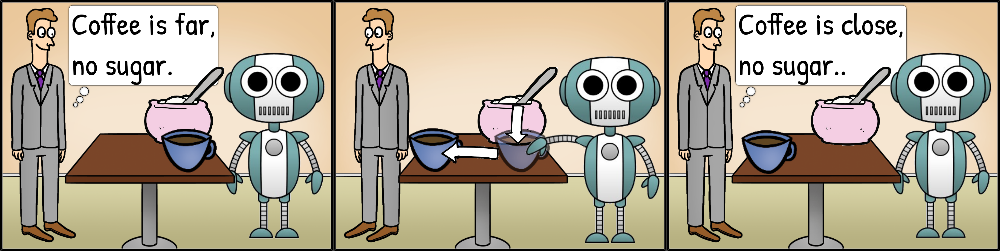
\includegraphics[width=0.9\linewidth]{figures/cartoon_inf_obs_bigger.png}
    \caption{
    % The robot adds sugar to the cup before pushing it while the human is not mindful. The position of the cup is \textit{observable}, so the human can update their belief after observing it. However, since sugar-in-cup is only \textit{inferrable}, and the human was not attentive (\textit{i.e.}, not ``co-present''), the human cannot tell whether sugar is added in the cup.
    % While  
    Human is not attentive when Robot adds sugar to the cup before pushing it forward. \textit{Assessing} the new situation after the two actions, Human can only ``know'' the cup's new position (\textit{observable}), but not \textit{SugarInCup} (\textit{inferrable}).
    }
    \label{fig:obs_attr}
\end{figure}

To better understand these observability classes, consider a scenario with a cup of coffee and some sugar on the table as depicted in Figure~\ref{fig:obs_attr}. 
Initially, the cup is far from the human and without sugar. While the human is not attentive (i.e., not \textit{co-present}, say) to the scenario, the robot adds some sugar to the cup and pushes it towards the human. 
Once the human is attentive again, they
can notice that the cup is closer. We can say that the position of the cup is \textit{observable}.
However, without observing the robot adding sugar, the human cannot know if some sugar is added to the cup. Hence, we say the \textit{SugarInCup} attribute is \textit{inferrable}, 
and the human agent would know if they observed the robot adding it. 

\section{Belief Updating}
An agent's belief can get updated in four ways as follows. 

\subsubsection{1. When Acting:}
If the agent executes an action, its belief is updated based on its effects. The state attributes appearing in the action's effect get updated with the new values, while the remaining attributes keep their same old values.

\subsubsection{2. When Being an Observant:}
\hspace{-0.05in}
\textbf{(\textit{Action Observability}.)}
An action executed by an agent is \textit{observed} by other agents \emph{co-present} throughout the action execution. Therefore, we state that if an agent observes an action getting executed, the agent will infer the \textit{inferrable} effects of the action.
Consequently, the agent immediately updates its belief state while each inferrable attribute affected by the action receives a new value.  

We do not yet consider cases where the robot's beliefs can diverge, too, assuming that, while not being observed, humans only make deterministic moves. Hence, regardless of the co-presence, the robot always updates its belief with both the \textit{inferrable} and \textit{observable} effects.

\subsubsection{3. Via Situation Assessment:}
The agent assesses the situation from its current location 
with the help of spatial reasoning and its reference frame, i.e., the formalized \textit{observability} model. Consequently, the agent updates its existing belief with the relevant ground truth. 

(Based on Definition~\ref{def:pssav}) We can always associate specific state attributes to \textit{places}. 
For example, suppose that being in the state $s_1$, the robot switches on the furnace placed in \textit{kitchen}, and this generates a new state $s_2$. Also, assume that
$f_{\textit{TurnOn}}
$ is $\observable$ (Definition~\ref{def:svof}).   
Then, the \text{place specific attribute function}, $f_{loc} : (...)$, w.r.t. the states
$s_1$ and 
$s_2$ can be expressed as, 
$f_{\textit{loc}} (f_{\textit{TurnOn}}^{s_1} )$ and $f_{\textit{loc}} (f_{\textit{TurnOn}}^{s_2} )$, respectively, and both map to $\textit{kitchen} \in Places$.

Consider the following scenario: The search progresses from $s_2$, along $s_1, s_2, ...$, such that the next action applicable in it is, the agent $(\varphi_h)$ \textit{moving} to the kitchen. This generates a new state $s_3$, and hence $f_{\textit{loc}} (f_{\textit{AgtAt}}(\varphi_h, s_3) )$ maps to $kitchen$, but so does  $f_{\textit{loc}} (f_{\textit{TurnOn}}^{s_3})$. 
In such cases, $\varphi_h$ assesses the \textit{status} of the furnace, i.e., the exact value of $f_{\textit{TurnOn}}^{s_3}$ in $s_3$, which is {\sc on}, and hence the human agent updates their belief.  

Note that the robot is always aware of the ground reality hence, technically, the idea 
is effective only for the human agent. Here, the robot takes the human's perspective and performs spatial reasoning as per the human's frame of reference or their current location in the environment. 
The human's belief is updated w.r.t. what they can see as ground truth (mimicked by the robot).
This enables $\varphi_h$ to learn an \textit{observable} attribute's value achieved earlier by the robot.

The agent updates its belief with relevant ground truth learned via situation assessment, performed ``immediately'' after the execution of each action. 
Hence, the robot performs situation assessment for the human and itself.

\subsubsection{4. When Being Communicated:}
Its belief gets updated by learning ground truth when another agent communicates an attribute-value pair. Communication occurs via a \textit{distinct set} of actions, modeled as a predefined communication protocol for a pair of sender-receiver agents. 

As the robot is always aware of ground truth, again, technically, it is effective only for the human belief.
We note that each action communicates only {\em one} attribute-value pair, so just one attribute gets updated in the human belief.

\subsubsection{Updates Workflow}
For each action, post its execution, the workflow for updating agents' beliefs is: (1.) the acting agent's belief is updated; (2.)
for the co-present agents, their beliefs are updated based on what they \textit{infer};
and (3.) \textit{situation assessment} updates their beliefs with respective \textit{observable} facts. 
To update initial observable facts, first, a dummy action is executed with no precondition and effect.

\section{Reasoning on Human Mental State}
The human and robot agents carry individual, distinct belief states w.r.t. the ground truth ($s$) (s.t. $\mathit{B}_{\varphi_r}^s$ is aligned with it), while the two can be either different or aligned. 
However, the agents act as if they are certain about their knowledge.  
Since the robot plans for both, it reasons about their distinct beliefs and manages the evolution of their individual beliefs. E.g., the robot adding salt to the pasta while the human being co-present or not can grow their belief states differently. 

To produce a legal joint-plan, the robot is fine with such a divergence unless it has an \textit{adverse} effect, e.g., the human acting based on their false belief.
At a stage, if the human agent, based on $\mathit{B}_{\varphi_h}^{s_i}$, can perform a set of actions that differs from what they could perform w.r.t. to $\mathit{B}_{\varphi_r}^{s_i}$ (or the ground reality), then we say that such divergent beliefs are \textit{relevant} to be \textit{tackled}.
A divergence is also declared as \textit{relevant} if an action has different effects w.r.t. the other agent's belief.

One approach to tackle it could be to trace back to the action that creates this divergence and {\em DELAY} it for future, if and when possible. E.g., the robot delays adding salt until the human arrives in the kitchen. 
Second, communicating relevant divergences to the human agent, and it is our main focus in this work. (However, delaying may not always find a solution, but it could reduce communication requirements. Our pilot development and results are in \textit{Appendix~C}.)

Assessing the impact of different human actions (based on their wrong $\mathit{B}_{\varphi_h}^{s_i}$) or effects, with their overall positive and detrimental impacts on achieving a joint task can be interesting.
An approach can be to analyze the agents' plan history or future actions to decide whether their beliefs should get aligned or not, or for that matter, how much to communicate, but it is out of the scope of this work. 

\section{Planning With Communication Actions}
We establish protocols between each \textit{sender-receiver} agents pair for communication, 
and model explicit communication actions between them. 
Note that these actions are different than agents' (non-) primitive actions.

\subsection{Modeling Communication Actions} 
Suppose there exists a state-variable function, $f_{svs}:(?g_1 (gr_1), ?g_2 (gr_2), ..., ?g_k (gr_k),\mathcal{S}) \rightarrow ?g_{k+1} (gr_{k+1})$ such that,
for the current world state $s \in \mathcal{S}$, the corresponding state attribute, $f_{\textit{svs}}(g_{(1)l},g_{(2)m},...,g_{(k)n},s)$ maps to $q$.

An agent $\varphi_i$ can communicate this attribute-value pair to another agent $\varphi_j$, if the following conditions meet as action precondition: 
(1.) For $\varphi_i$, its belief state satisfies the fact being communicated, i.e.,
$f_{\textit{svs}}(g_{(1)l},g_{(2)m},...,g_{(k)n},B_{\varphi_i}^s) = q$, and (2.) $\varphi_j$'s belief state does not satisfy this truth, i.e., $f_{\textit{svs}}(g_{(1)l},g_{(2)m},...,g_{(k)n},B_{\varphi_j}^s) = r$ such that $r \neq q$.
The effect of this action is that now 
$\varphi_j$'s belief is updated, i.e., $f_{\textit{svs}}(g_{(1)l},g_{(2)m},...,g_{(k)n},B_{\varphi_j}^s) \leftarrow q$. 

\subsection{The New Planning Approach}

At this stage, say, the ground truth ($s_i$), we assume \textit{Updates Workflow} was already called, and then the sender reasoned out and decided to \textit{tackle} the receiver's divergent beliefs. 

    % \item \textbf{Relevant Belief Divergence.}
    % At a given stage, if the human agent, based on their own belief, can perform a set of actions that differs from 
    % the one 
    % the human :could perform w.r.t. to the robot's belief (or the ground reality), then we say that such divergence in their belief is \textit{relevant}.
    % % 
    % A divergence is also declared as \textit{relevant} if an action has different effects w.r.t the other agent's belief.
    % However, currently, our reasoning system is myopic: We do not evaluate in a principled way the impact of \textit{different} actions that humans could execute (based on their wrong belief), or of \textit{different} effects, with their overall positive and detrimental effects on achieving the joint task. At this stage, it simply ``decides'' to align the agent's beliefs using communication actions whenever the belief divergence is relevant.
    % However, a smarter approach might be to analyze the history of plan trace(s) or agents' future actions to decide whether their beliefs should get aligned or not, or for that matter, how much to communicate, but it is currently out of the scope of this work. 
    % This we intend to tackle in future.
    % .  
    % But, for now, 
    
    % \item \textbf{Communicate Only The Required Facts.}
    \subsubsection{Communicate Only The Required Facts.}
    % The new approach 
    % Decides only the essential changes in the receiver's belief to be made. 
    Note that there exists at least one \textit{attribute}-\textit{value} in receiver's belief state causing adverse effects. 
    The approach, explained in the next \textit{three} steps, looks for the minimal number of such attribute-value pairs to be communicated so that
    % its modified belief (updated, but could still be diverging) becomes \textit{irrelevant}. 
    the divergence in the updated belief is made \textit{irrelevant}, or even eliminated.
    % And, for that following steps are followed. 
    % In the worst case, the robot communicates all the divergent attribute-value pairs, and their belief states are perfectly aligned. 
    % The subroutine used to decide which all communication actions will appear in the sender's executable plan; is described in the following steps:
    \begin{enumerate}
        \item 
        \textit{Store} each attribute and its value if the attribute's value differs in the receiver's belief from the sender's belief. 
    
        \item For them, \textit{build} actions, $\textit{comm-action}_i$, following the schema described earlier. Say, they are equally costly.  
        
        \item 
        % At a given stage of planning, e.g., the ground truth $s_i$, 
        (Follow Breadth-First Search) 
        The \textit{source} is $B_{\varphi_h}^{s_i}$, and each $\textit{comm-action}_i$ changes and aligns \textit{exactly} one attribute while its updated value satisfies the ground truth. If $\textit{comm-action}_i$ is applied, generates a new belief state (following the regular state transition rules), using: $B_{\varphi_h}^{s_i,1} = \gamma(B_{\varphi_h}^{s_i}, \textit{comm-action}_i)$.
        It continues until the first (updated) belief is selected to expand s.t. its remaining divergence is \textit{ineffective}. We then \textit{retrieve} all the actions used from the root until the current belief state.   
    \end{enumerate}

These retrieved actions are appended to the sender's plan.

\section{Formal Properties}
Note that our solver has a similar high-level elaboration process, i.e., its underlying mechanism, as the old solver but with a better estimation of the evolution of agents' beliefs.  
However, when discussing its soundness and completeness, dependent on the soundness and completeness of the underlying mechanism, we must distinguish between the problem specifications used by these solvers. 

In the worst-case, our specifications would pick each $p \in P$ (all propositions), generate a new set of primitive propositions for every possible combinations of $|\{\observable,\inferrable\}| \times |\mathit{Places}|$. 
So, the size of the new encoding for primitive propositions is worst-case \textit{linear} in the size of $P$.

For the old specifications and to support the old solver's simplified assumptions, an equivalent encoding to the above can be considered $p$ belonging to the $\inferrable$ class for every $place \in \mathit{Places}$, and the agents can \textit{always} be considered co-present.  
Note that for a domain like Blocksworld where explicit modeling of $\mathit{Places}$ is not required, it considers a \textit{single} dummy place $p_{du}$ (depicting that everything occurs here) to serve this new encoding. So, it \textit{ensures} that transformed formalism captures everything that can be formulated using the original dual-HTNs but technically provides a latitude to model more realistic problems. 

\begin{theorem}
\textbf{(Soundness.)} The new solver is sound.
\vspace{-0.06in}
\begin{proof}
Following Definition~\ref{def:joint-sol-plan},
we show that the joint solution plan generated is executable:
For a branch, it is guaranteed that it meets the {\em solution conditions}.
Moreover, each precondition for an agent's action is achieved in earlier time stamps by either: its own action, 
\textit{inferred} while observing another agent's actions, 
another agent \textit{communicated},
or it is \textit{assessed} by observing a situation and reasoning.
Of course, another agent’s action supplying the precondition, an attribute (in $\observable$) and its value, cannot be destroyed. 
Hence this branch/trace is executable.

Finally, since the human can make any choices during execution,
and are unknown upfront, any of its branches, by the
above argument, will be executed. 
Implies, the joint solution plan is executable.
\end{proof}
\end{theorem}

\begin{theorem}
\textbf{(Completeness.)} The new planning algorithm is complete, provided the underlying mechanism can exhaustively generate all possible plan elaborations. 
\vspace{-0.06in}
\begin{proof}
Suppose a problem modeled based on our formalism has a solution, say, a joint solution tree, $\tau$ and is sound. 
From $\tau$, remove all the communication and situation assessment steps, and say it generates $\tau'$. Now, relax the original problem, considering all the agents being always co-present and making all the propositions \textit{inferrable} everywhere. 
Technically, the solver will generate $\tau'$ for this new problem when it exhaustively generates the whole search space (of course, it may contain redundant actions). 
We assure it believing on the underlying mechanism and that there is at least one solution ($\tau$) for the original problem. As a result, it is trivial to visualize that $\tau'$ is always extendable to generate $\tau$ w.r.t. the original problem. (\textit{Updates Workflow}.) After the execution of each step, one can employ the situation assessment and action's effect inference subroutines, checking for belief divergences and using communication actions if needed. 
\end{proof}
\end{theorem}

\begin{figure}[t!]
    \centering
    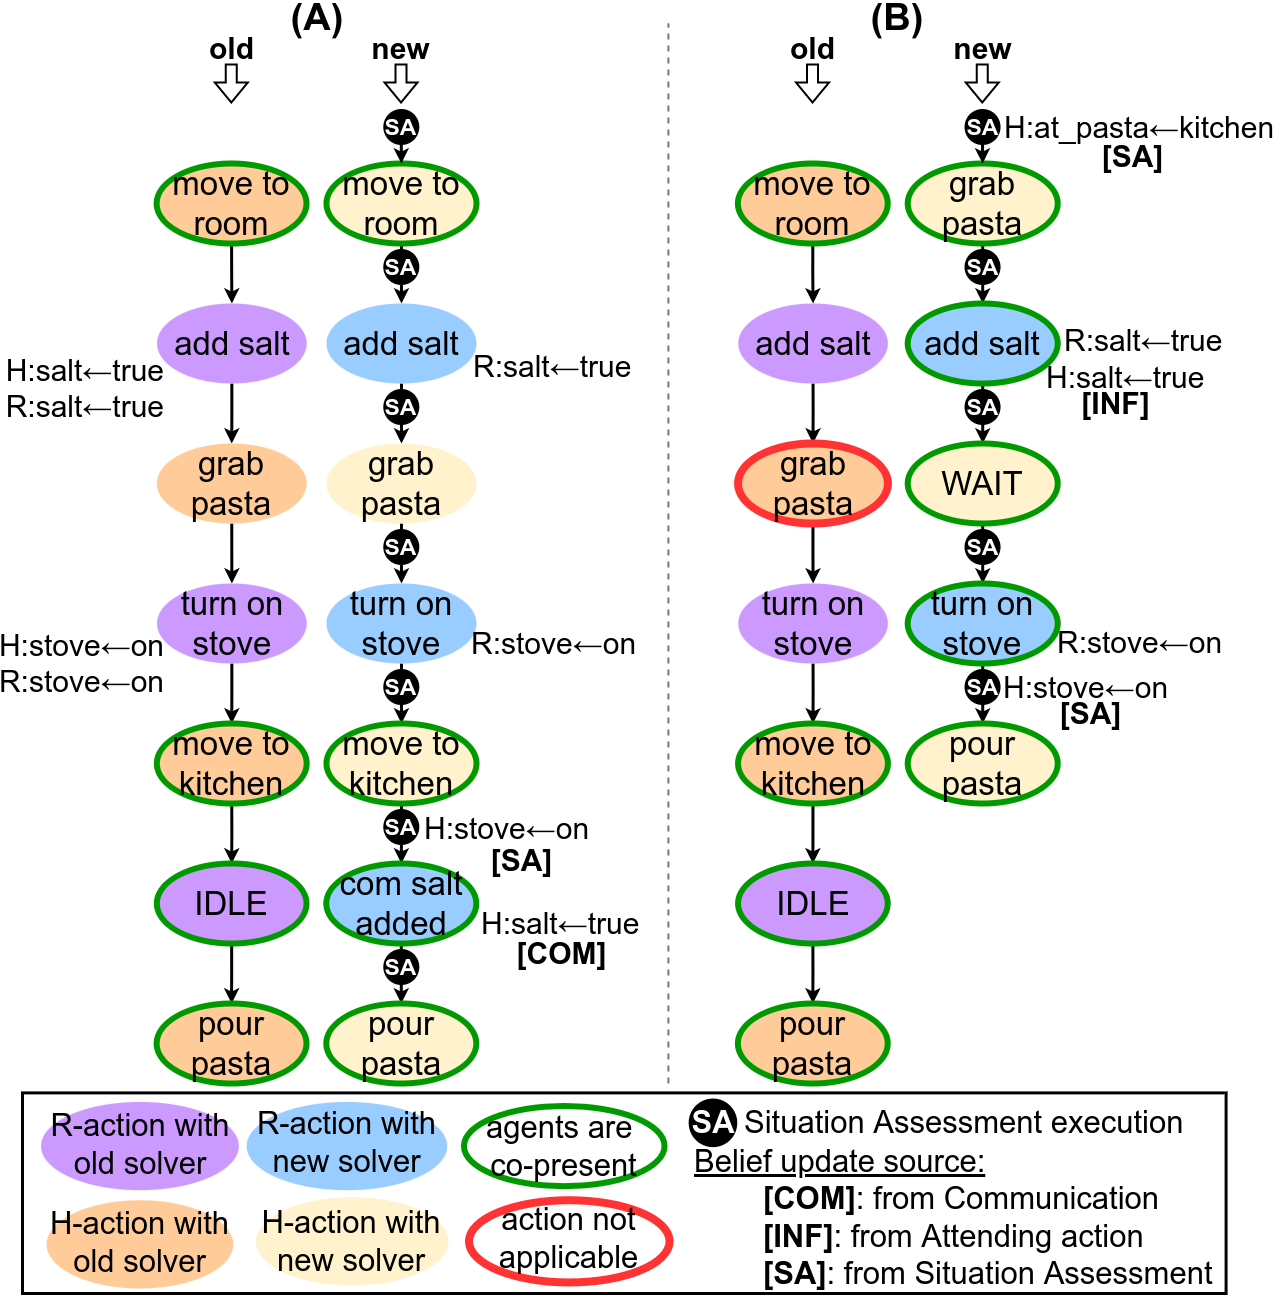
\includegraphics[width=0.99\linewidth]{figures/bc_plans.png}
    % \includegraphics[width=0.85\linewidth]{figures/new_plans.png}
    \caption{
    Plans obtained in two scenarios: Each presents two plans. (\textit{Left}) Obtained by the old solver, and (\textit{Right}) obtained by ours. The latter depicts more realistic and appropriate belief updates (focusing on two attributes).
    Case~(A): the human has no certainty on {\em SaltInPot}, while ours decides to communicate to remove the ambiguity. 
    And, Case~(B): an initial belief divergence on {\em AtPasta} induces an ``invalid'' plan, but ours predicts that the human \textit{assess} the pasta location and update their belief, without being communicated.
    }
    \label{fig:scenarios}
\end{figure}

    

\section{Empirical Evaluation}

Before we describe three {\em novel} domains used in the experiments and the results to compare the old and new approaches, let us make a ``high-level'' distinction between the two. 
In principle, the old solver can handle a belief divergence only when agents start with unaligned, distinct beliefs. But, when it is not so, unlike ours, it assumes that the agents' beliefs never diverge during planning, and hence there is no way it can handle a divergence created by an agent in practice. 
The old solver can align the beliefs via explicitly influencing (the human's) action model and a cumbersome technique using triggers to update their task networks. Our approach estimates the evolution of belief divergences at planning time and uses explicit communication actions to handle them in practice to generate robust plans. 

\subsubsection{Cooking Pasta Domain:}
Suppose a stove and salt are available in \textit{Kitchen} $\in$ $\textit{Places}$, and the pasta can be either in \textit{Kitchen} or \textit{Room} (the two are adjacent). The agents have different roles and can only operate in the two places. Robot \textit{adds} salt to the pot and \textit{turns-on} the stove. Human \textit{grabs} the pasta and \textit{pours} it into the pot. 
Pasta can be poured after salt is added to the pot and the stove is {\sc on}.
Focus on the following two attributes associated to \textit{Kitchen}: For a given state, $s_i \in \mathcal{S}$, $f_{\textit{SaltInPot}}^{s_i} \in \{\textit{true, false}\}$ and $f_{\textit{stove}}^{s_i} \in \{\textit{on, off}\}$ such that only $f_{\textit{stove}}^{s_i}$ is \textit{inferrable}, all others belong to $\observable$.

\subsubsection{Preparing Box Domain:}
A box filled with a fixed number of balls with a sticker on it is considered prepared and needs to be sent. Both the agents can \textit{fill} the box with balls from a bucket, while only the robot can \textit{paste} a sticker and only the human can \textit{send} the box. The bucket can run out of balls, so when only one ball is left, the human \textit{moves} to another room to \textit{grab} more balls and \textit{refill} it. 
The number of balls in the box is \textit{inferrable}, while all other variables are {\em observable}. 

\subsubsection{Car Maintenance Domain:}
The washer fluid ($\observable$) and engine oil ($\inferrable$) levels have to be \textit{full} before \textit{storing} the oil gallon in the cabinet ($\inferrable$). 
Only the robot can \textit{refill} both the tanks and store the gallon while situated at \textit{Front} of the car. 
\textit{Front-left} and \textit{Front-right} headlights have to be \textit{checked} and a light-bulb has to be \textit{replaced} at \textit{Rear}. 
Only the human can check and replace lights, and they can start with either of these two tasks.
Both agents starts at \textit{Front}.
The car's hood needs to be \textit{closed} by the human at last.

\subsection{Experiments}

\subsubsection{Qualitative Analysis}

In the first domain, we highlight \textit{subtleties} the old solver overlooks and how ours is aware of them, updates beliefs, and effectively manages divergences. 
We discuss the plans obtained in two scenarios 
as shown in Figure~\ref{fig:scenarios}. Assume that both the agents are in \textit{Kitchen} and the human acts first. Scenario~(A): Captures the agents' plans when the pasta is in \textit{Room}. 
Scenario~(B): 
In hindsight, the pasta is moved from \textit{Room} to {\em Kitchen}, which the robot knows, while the human still has the old belief.

\begin{itemize}
    % \item \textbf{Scenario~(A):} 
    % Although the solvers generate similar plans, they update the human's belief differently if and when the human and robot are co-present. E.g., turning on the stove ideally (realistically) does not affect the human's mental state, which is not the case for the old solver. It considers agents omniscient, so the human knows everything immediately once achieved. 
    % Our solver predicts it when the human returns to the kitchen and assesses that the stove is {\sc on}, and their belief gets updated.
    \item \textbf{Scenario~(A):} 
    % The human leaves the kitchen and hence practically is unaware of the changes achieved in the environment by the robot's actions: {\em turn on} and {\em add salt}. 
    As the human left {\em Kitchen}, practically, they are unaware of the changes caused by the robot's actions: {\em turn on} and {\em add salt}. (\textit{Left}) The old solver considers agents omniscient. So, the human knows that the stove is {\sc on}, and salt is added even before arriving back in {\em Kitchen}. (\textit{Right}) Thanks to both situation assessment and inference based on action observability, it estimates that when returning to the kitchen, the human assesses that the stove is {\sc on}. Moreover, it predicts that the human cannot know \textit{SaltInPot} and that this divergence, identified as relevant, needs to be handled via communication.
    % The old solver considers agents omniscient, i.e., they know everything immediately once achieved. Hence, the human knows that the stove is {\sc on}, and salt is added even before being back in \textit{Kitchen}.
    % The new solver, thanks to both an appropriate situation assessment and inference based on action observability, estimates that when returning to the kitchen, the human assesses that the stove is {\sc on}.
    % Moreover, it predicts that the human cannot know the \textit{SaltInPot} fact and that this divergence, identified as relevant, needs to be handled via communication. 
    % This divergence was ineffective after the robot communicates it to the human.
    \item
    % \textbf{Scenario~(C):} In the updated scenario, using the old approach, the human moves to \textit{Room} to grab the pasta, but in reality, the action \textit{fails} as it is not a legal action w.r.t. the robot's belief or the ground truth. But, the way our planning system works, the human agent assesses the
    \textbf{Scenario~(B):}
    % With the old solver, 
    (\textit{Left}) the human moves to \textit{Room} to \textit{grab} the pasta, but in reality, being an illegal action w.r.t. 
    % the robot's belief or 
    the ground truth, it \textit{fails}. 
    (\textit{Right}) the human agent \textit{assesses} the environment to update their beliefs, knowing \textit{PastaInKitchen}. 
    % Also, no communication is required for this update. 
    Hence, no communication is required.
    % environment and updates their belief state, knowing that the pasta is in the kitchen. Hence no communication is required to align their belief. The rest is self-evident.
\end{itemize}

\begin{table}
    \begin{adjustbox}{width=0.77\columnwidth,center}
    \begin{tabular}{@{}c|r r r| c@{}}
        % \hline
        \multirow{2}{*}{
        \textbf{Domain}} & \multicolumn{3}{c|}{\textbf{\textit{Old Solver}}} & \multicolumn{1}{c}{\textbf{\textit{Our Solver}}}
        \\
        % \cline{2-6}
        & \multicolumn{1}{c}{\textit{S}} & \multicolumn{1}{c}{\textit{NA}} & \multicolumn{1}{c|}{\textit{IDL}} & \multicolumn{1}{c}{\textit{Com}} 
        \\ \cline{1-5}
        \textit{Cooking} & 18.6\% & 77.0\% & 23.0\%  & 54.9\%\\
        \textit{Box} & 25.0\% & 83.3\% & 16.7\%  & 68.8\%\\
        \textit{Car} & 12.5\% & 73.2\% & 26.8\%  & 79.7\%\\
        \hline
        \textbf{Average} & 18.7\% & 77.8\% & 22.2\%  & 67.8\%\\
    \end{tabular}
    \end{adjustbox}
    \caption
    {
    \label{tab:q_results}
    % Comparison of the two solvers on the two domains. 
    % In each domain: 
    For the \textit{old solver}, the success rate (\textit{S}), the ratio of failed plans due to a non-applicable action (\textit{NA}), and the ratio of failed plans due to an inactivity deadlock case (\textit{IDL}), while for \textit{our solver}: (the success rate is always 100\%), the ratio of plans including a communication action (\textit{Com}).
    }
\end{table}

\subsubsection{Quantitative Studies}

Quantitative results in three new domains appear in Table~\ref{tab:q_results}. 
We consider (in box domain) \textit{three} boxes to be prepared and sent. 
In each domain, we generated 512 different initial states, including 448 (87.5\%) with divergent initial beliefs and 64 states where beliefs are fully aligned initially. 
Overall, 3072 plans were generated.

With the old approach, a planning failure occurs due to: 
(a) an action of a plan not applicable in another agent's belief state, including the ground truth; 
(b) if an inactivity deadlock occurs, which is assumed to be the case after a succession of at least four {\em WAIT} and (or) {\em IDLE} actions. 
Such deadlocks occur when the human has a belief divergence and waits for a never-happening robot's action, e.g., waiting for \textit{adding} salt, but \textit{SaltInPot} is already achieved.
For the old solver, the success rate (\textit{S}), the \textit{ratios} of the number of failed plans due to a inapplicable action (\textit{NA}) and to an inactivity deadlock (\textit{IDL}) appear in the table.
For ours, the \textit{ratio} of successful plans with a communication action is presented under \textit{Com}.

As the old solver does not handle belief divergence in planning, the applicability of actions is never an issue w.r.t. another agent's beliefs. 
Therefore, if the \textit{IDL} case occurs, it is understood that the initial belief divergences are not tackled by modeling triggers explicitly in the task specifications. 

Our solver always finds legal plans, and on average $\approx$ 68\% of them use \textit{communication}.
Moreover, the robot doesn't need to communicate systematically as assessing situations handles a major part of the divergences (87.5\% of the scenarios have divergent beliefs initially).
For the old solver, if no initial belief divergence exists, it always finds a legal plan, considering the agents omniscient. 
E.g., Fig.~\ref{fig:scenarios}(A). However, sometimes, this causes problems in practice.
Scenarios beginning with unaligned beliefs induce actions often not applicable in another agent's belief state (or the ground truth), evident by the (average) 18.7\% success rate.

We can see that our solver uses more communication actions in the car maintenance domain than in the other two.
But looking at the \textit{low} old solver's success rate (12.5\%), we conclude that this domain generally needs more communication. 
Compared to others, it purposely creates non-relevant belief divergence, e.g., the robot storing the gallon in the cabinet ($\inferrable$) is irrelevant.
After a close analysis, we found that $\approx$ 42\% of the plans have divergent human beliefs at least in one branch after the last action (\textit{leaf}) was executed (i.e., \textit{irrelevant} divergences never got communicated). 

\section{Discussion}
We formalize execution-time observability conventions based on situation assessment and action observability (ToM). We use it to estimate the evolution of the human mental state and capture belief divergences. 
A new planner is described, which utilizes this better estimation of human mental state to plan for more robust and consistent human-robot joint activities such that a relevant belief divergence is tackled by explicitly modeled communication actions. 

Moreover, our effort was to make our main \textit{contributions} (i.e., formalizing observability based conventions) to have a ``generic'' description. Hence, they are not limited to only our intended framework (HATP/EHDA).

Handling these conventions formally is vital for robust planning, as otherwise, it can lead to problems at run-time. 
E.g., Fig.~\ref{fig:scenarios}(A): the human knowing \textit{SaltInPot} is ambiguous. 
Explicit reasoning on the human mental state detects ambiguous situations and removes them via communication. 

Our formalism does not refute something believed by an agent through situation assessment. 
E.g., for some $s_i \in \mathcal{S}$, if the human \textit{wrongly} believes that the pasta is in \textit{Kitchen}. The situation assessment does not help refute this, while the human is in \textit{Kitchen}. 
The reason is that $f_{\textit{PastaNotInKitchen}}^{s_i}(...)$ is not modeled explicitly as an attribute. 
And hence such issues do not affect the completeness. 
Moreover, our solver handles them as a \textit{relevant} divergence to be aligned. Followed by the human is communicated with correct updates.

\bibliography{bib.bib}

\end{document}

